\documentclass[a4paper, 12pt, twoside]{article}
\usepackage[utf8]{inputenc}	
\usepackage[T1]{fontenc}		
\usepackage[francais]{babel}
\usepackage{lmodern}
\usepackage{ae,aecompl}
\usepackage[top=2.5cm, bottom=2cm, 
			left=3cm, right=2.5cm,
			headheight=15pt]{geometry}
\usepackage{graphicx}
\usepackage{eso-pic}
\usepackage{array} 
\usepackage{hyperref}
\usepackage{lastpage}
\usepackage{listings}

%%%%%%%%%%%%%%%%%%%%%%%%%%%%%%%%%%%%%%%%
%    Page de garde (Pagedegarde.tex)   %
%%%%%%%%%%%%%%%%%%%%%%%%%%%%%%%%%%%%%%%%
% Haseeb Chaudhry, 2019
\usepackage{fancyhdr}
\usepackage{nomencl}
\makeatletter
\def\@ecole{école}
\newcommand{\ecole}[1]{
  \def\@ecole{#1}
}

\def\@entreprise{Nom de l'entreprise}
\newcommand{\entreprise}[1]{
  \def\@entreprise{#1}
}

\def\@datedebut{\today}
\newcommand{\datedebut}[1]{
  \def\@datedebut{#1}
}


\def\@datefin{\today}
\newcommand{\datefin}[1]{
  \def\@datefin{#1}
}



\def\@specialite{Spécialité}
\newcommand{\specialite}[1]{
  \def\@specialite{#1}
}

\def\@ED{\'{E}cole Doctorale}
\newcommand{\ED}[1]{
  \def\@ED{#1}
}

\def\@doctorat{Doctorat}
\newcommand{\doctorat}[1]{
  \def\@doctorat{#1}
}

\def\@adresse{Adresse}
\newcommand{\adresse}[1]{
  \def\@adresse{#1}
}

\def\@directeur{directeur}
\newcommand{\directeur}[1]{
  \def\@directeur{#1}
}

\def\@fonction{Développeur }
\newcommand{\fonction}[1]{
  \def\@fonction{#1}
}

\def\@encadrant{encadrant}
\newcommand{\encadrant}[1]{
  \def\@encadrant{#1}
}
\def\@jurya{}{}{}
\newcommand{\jurya}[3]{
  \def\@jurya{#1,	& #2	& #3\\}
}
\def\@juryb{}{}{}
\newcommand{\juryb}[3]{
  \def\@juryb{#1,	& #2	& #3\\}
}
\def\@juryc{}{}{}
\newcommand{\juryc}[3]{
  \def\@juryc{#1,	& #2	& #3\\}
}
\def\@juryd{}{}{}
\newcommand{\juryd}[3]{
  \def\@juryd{#1,	& #2	& #3\\}
}

\makeatother

\newcommand\BackgroundPic{%
	\put(0,0){%
		\parbox[b][\paperheight]{\paperwidth}{%
			
\includegraphics[height=0.45\paperheight]{resources/Bordure.png}%
			\vfill
		}
	}
}
\newcommand\EtiquetteThese{%
	\put(0,0){%
		\parbox[t][\paperheight]{\paperwidth}{%
			\hfill
			%\colorbox{blue}{		
				\begin{minipage}[b]{2em}
					
\includegraphics[width=4.0\textwidth]{resources/logo_miage.png}\\					
					%\centering\Huge\textcolor{white}{M\\I\\A\\G\\E\\}
					\vspace{0.2cm}
				\end{minipage}
			%}
		}
	}
}

\makeatletter
\newcommand{\pagedegarde}{
\newgeometry{top=2.5cm, bottom=1cm, left=2cm, right=1cm}
\AddToShipoutPicture*{\BackgroundPic}
%\AddToShipoutPicture*{\EtiquetteThese}
  \begin{titlepage}
  \centering
      
\includegraphics[width=0.5\textwidth]{resources/logo_Paris_Nanterre_couleur_RVB.png}
      \hfill
      
\includegraphics[width=0.40\textwidth]{resources/logo_entreprise.png}\\
    \vspace{1cm}
    \vspace{1cm}
      {\huge 
      	{\bfseries Rapport de stage}\\
    \vspace{0.5cm}}
      	M1 MIAGE, parcours classique\\
    \vspace{1cm}
   		
    \vspace{1cm}
    	{\huge\color{red!75}\bfseries{\@title}}\\
    \vspace{0.5cm}
    {\bfseries Entreprise d'accueil : \@entreprise}\\
    {\bfseries Stage réalisé du \@datedebut\ au \@datefin}\\
    %	{\Large{\bfseries Spécialité doctorale ``\@specialite''}}\\
    \vspace{2cm}
    	\textit{présenté et soutenu par}\\
    \vspace{0.5cm}
    	{\Large {\bfseries \@author}} \\
    \vspace{0.5cm}
    	le \@date \\
    \vfill
     %  {\LARGE \color[rgb]{0,0,1} \bfseries{\@title}} \\
    %\vfill
      %  Directeur de thèse : {\bfseries \@directeur}\\
       % Co-encadrant de thèse : {\bfseries \@encadrant}\\
    %\vfill
	\begin{tabular}{>{\bfseries}lll}
		\large Jury de la soutenance\\
		\vspace{0.15cm}\\
		\@jurya
		\@juryb
		\@juryc
		\@juryd
	\end{tabular}
	%
\includegraphics[width=0.20\textwidth]{logo_entreprise.png}\
	\vfill
	
	%\@adresse
  \end{titlepage}




\restoregeometry  
\makenomenclature

\pagestyle{fancy}

\renewcommand\headrulewidth{1pt}

\fancyhead[L]{\@fonction}

\fancyhead[R]{\@entreprise}


\renewcommand\footrulewidth{1pt}

\fancyfoot[L]{\@author}

\fancyfoot[C]{}

\fancyfoot[R]{ Page \thepage/\pageref{LastPage}}
}



\author{Haseeb Chaudhry}
\title{Stage de Consultant fonctionnel}
\entreprise{Sopra Banking Software}
\fonction{Consultant fonctionnel}
\datedebut{01 avril 2019}
\datefin{26 juillet 2019}

\date{Mardi 02 juillet 2019}
\jurya{M. Pascal Poizat}{Professeur des universités}{Responsable de promotion}
\juryb{Mme Martha Rukoz}{Professeur des universités}{Tuteur enseignant}
\juryc{M. Alexandre LIGER}{Responsable Pôle Service Anadefi}{Maître de stage}

\begin{document}

\pagedegarde

\section*{Remerciements}
Je tiens à remercier mon maître de stage, Alexandre LIGER, pour son
accueil, le temps passé ensemble et le partage de son expertise au quotidien et pour la confiance qu'il m'a accordée tout au long de mon stage. Grâce à lui j'ai pu m'épanouir dans les missions qu'il m'a confiées, grâce à qui, j'ai pu découvrir un autre aspect de l'informatique, pour ses nombreux conseils sur mon avenir professionnel. Je garde une très bonne expérience au sein de Sopra Banking Software et je suis très reconnaissant envers lui.\\

Je tiens à remercier Irenee MANGENOT pour m'avoir accueilli à Montpellier, pour m'avoir guidé, formé durant toute une semaine mais également pour m'avoir apporté son aide si précieuse sur tous les projets sur lesquels nous avons pu travailler ensemble et je le remercie pour sa bonne humeur.\\

Je tiens à saluer Christophe ROUXEL et Simon LABATUT pour leur patience durant ma formation, de m'avoir apporté une aide technique et fonctionnel sur nos projets en commun.\\

Un grand merci à Aurélie BEREAU ADELISE et Thierry-Michel BARRAL ainsi qu'à toute leur équipe pour m'avoir invité à leur daily stand-up.\\

J'aimerais aussi remercier Edouard MARINIER et Benoit COQUIL pour m'avoir donné la possibilité d'effectuer ce stage dans leur agence.

\newpage

%La table des matières
\tableofcontents

\section{Introduction}
Dans le cadre de ma première année de master MIAGE\footnote{Méthodes Informatique Appliqué à la Gestion des Entreprises} à l'université Paris Nanterre, nous devons effectuer un stage de fin d'année pour mettre en oeuvre tout ce que l'on a pu apprendre durant les cours, travaux dirigés et les projets. Ce Stage nous permet donc de valider notre année et d'assurer notre passage du master 1 au master 2.\\

Ayant un profil très technique par mes expériences professionnelles précédentes et naturellement plus orienté vers la programmation, j'ai voulu découvrir un autre aspect de l'informatique. Cela me permettrait d'élargir mes compétences, d'élargir mes connaissances dans le but d'avoir un profil plus polyvalent. Cela me permettrait également d'avoir du recul, car dans ma vie professionnelle future, j'interagirai avec différents métiers liés à l'informatique.\\

J'effectue donc un stage de quatre mois\footnote{Du 1er avril au 26 juillet} chez Sopra Banking Software où j'occupe le poste de consultant fonctionnel.\\

Ce rapport présente le travail effectué du 01 avril 2019 au 10 juin 2019 qui continuera jusqu'au 26 juillet 2019.\\

{Le plan du rapport se déroulera de la manière suivante :}\\
Tout d'abord, la présentation l'organisme d'accueil, présentation de l'outil, de l'équipe et le cadre du travail. Nous étudierons par la suite, le problème posé sur chaque projet et le travail effectué lors de mon stage.
\section{Présentation de l'entreprise}
\subsection{Sopra Steria}
En 2014 le Sopra Group fusionne avec l'entreprise Steria, deux très grandes entreprises dans le domaine des systèmes d'informations, Sopra Steria est un acteur majeur de la transformation numérique en Europe.
\textit{ Sopra Steria propose des prestations de conseil et des services technologiques (intégration de systèmes, gestion d’infrastructures, exécution de processus métier) et est un éditeur de logiciels métier (RH, banque, immobilier). L'entreprise compte plus de 37 000 collaborateurs et est présente à travers plus de vingt pays. Elle est surtout présente et reconnue en Europe notamment en France et en Angleterre où elle réalise la majeure partie de son chiffre d'affaire}.\\

Grâce à ses différentes filiales, Sopra Steria est présent sur de nombreux secteurs ainsi que dans de nombreux domaines :\\
\begin{figure}[h]
\centering
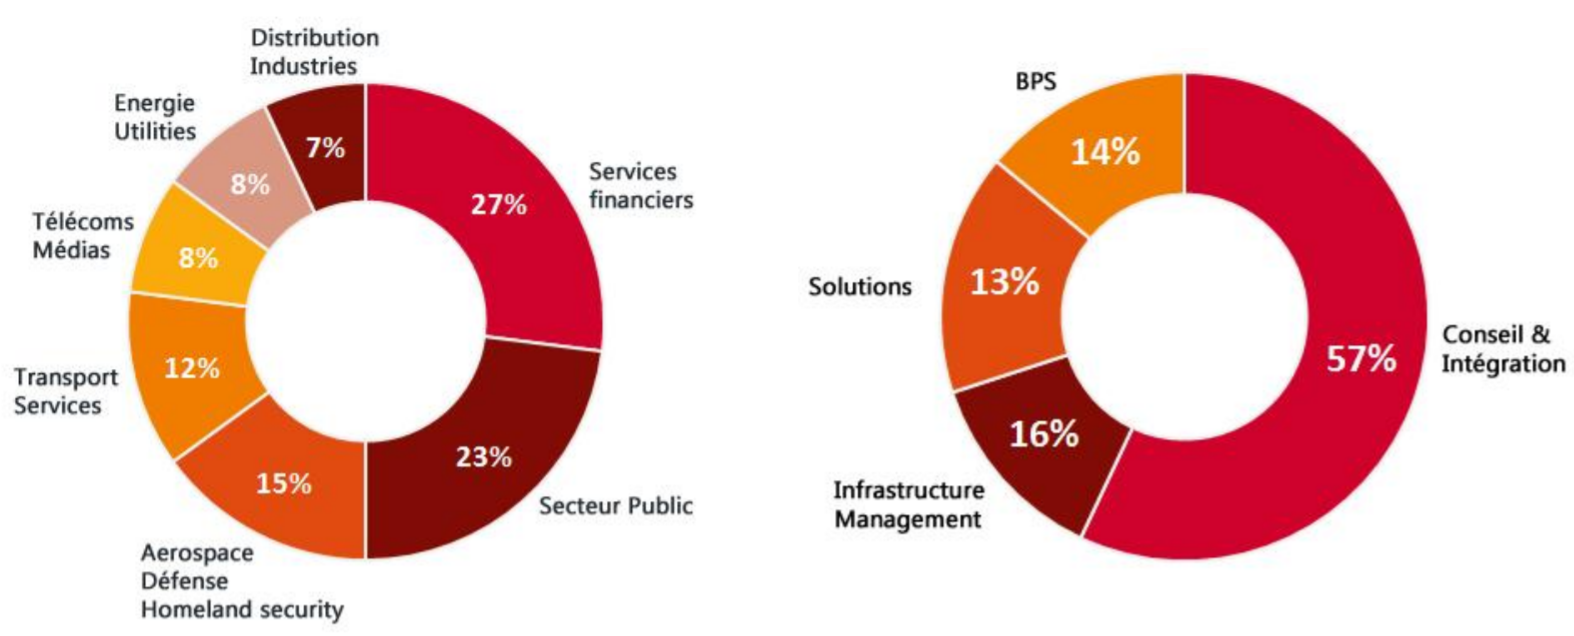
\includegraphics[scale=0.6]{resources/sopraSteriaGraph.png}
\caption{Secteurs et domaines d'activités de Sopra Steria}
\label{sopraSteriaGraph}
\end{figure}

Pour ma part, j'ai travaillé pour la filiale Sopra Banking Software.

\newpage
\subsection{Sopra Banking Software}
\textit{La transformation numérique entraîne un véritable bouleversement dans les organisations et les modes de travail, dans les pratiques managériales et dans l’engagement des collaborateurs.}\\

\textit{Sopra Banking Software est une filiale du groupe Sopra Steria, leader européen de la transformation numérique. Avec plus de 44 000 collaborateurs, ce dernier affiche un chiffre d’affaires 2018 de 4,1 milliard d’euros.}\\

\textit{Avec ses 4000 experts, un chiffre d’affaires 2018 de 373,7 millions d’euros et l’un des portefeuilles de solutions et de services les plus complets du marché, Sopra Banking Software est de longue date le partenaire de confiance de plus de 800 banques dans 70 pays.}\\

\textit{Son savoir-faire sans égal lui permet de répondre aux besoins d’innovation comme de développement de banques et institutions financières de toute taille et activité.\footnote{Source dans la webographie}}\\

Sopra Banking Software propose des solutions financières à destination des banques et des instituions financières. Elle est présente en Europe, Asie, Afrique et depuis peu en Amérique du nord. 


\begin{figure}[h]
\centering
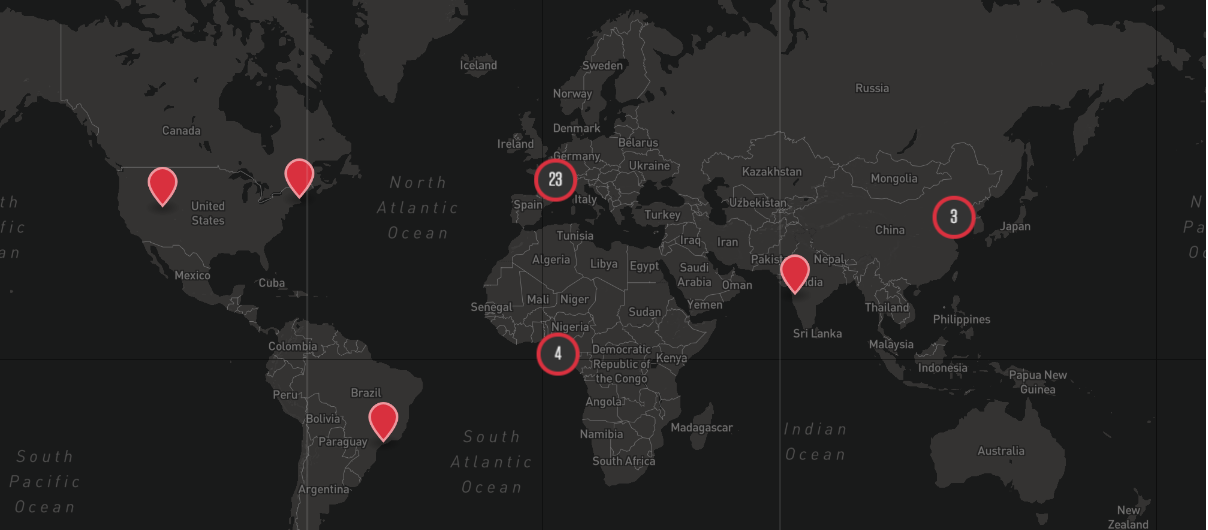
\includegraphics[scale=0.6]{resources/SBSImplantSites.png}
\caption{Implantation \& sites de Sopra Banking Software}
\label{SBSImplantSites}
\end{figure}

\newpage
\subsection{O.R. System}

\textit{O.R. System est un fournisseur de solutions et logiciels pour la gestion du risque de contrepartie, l’analyse financière et la notation interne. Avec plus de 300 000 utilisateurs dans 70 pays, nous sommes leaders sur notre marché. Nous nous engageons à agir comme partenaire pour chacun de nos clients, à créer de la valeur pour eux, et nous nous adaptons constamment à leurs marchés et besoins.}\\

\textit{Afin d’accompagner ses clients O.R. System a une équipe de spécialistes multidisciplinaires : experts métiers (analyse financière et notation), chefs de projets, experts produits, architectes techniques, et formateurs.
Créée en 1985, O.R. System débuta en tant qu’éditeur de logiciel dédié aux banques et institutions financières.
La première version de son produit phare ANADEFI fut développée et implémentée au début des années 90 : un outil puissant d’analyse financière afin d’aider les institutions financières à évaluer leurs clients et contreparties.}\\

\textit{Avec le développement rapide des réglementations Bâle I et II, d’un pur outil financier ANADEFI s’est transformé en plateforme complète supportant l’implémentation de toute méthode de notation interne.}\\

\textit{En 2005, O.R. System lance une version d’ANADEFI dédiée aux Banques Centrales leur fournissant une solution complète pour la gestion de leurs informations financières, et de leurs bases de données risques et incidents de paiement.}\\

\textit{Sopra Banking Software rachete O.R System en 2019.
Cette acquisition permet à la nouvelle équipe de donner un nouveau départ à l’entreprise et d’accélérer sa croissance, en France comme à l’international.
L’un des objectifs de la nouvelle direction est de développer ses parts de marché à l’international et de nouvelles offres dans le domaine de la gestion de risques de contrepartie.\footnote{Source dans la webographie}}\\

Sur le plan organisationnel, le siège social est désormais à la tour Manhattan située à la Défense mais elle conserve les équipes techniques et administratives sur Montpellier. Plusieurs agences\footnote{Les équipes de Sopra Banking Software sont reparties par agence.} vont s'occuper des différents pôles d'Anadefi.



\section{Anadefi}
\subsection{Présentation d'Anadefi}
Anadefi est le progiciel leader en France pour l’analyse financière de comptes d’entreprises s’appuyant sur près de quinze ans d’existence et d’expérience. Conçu spécifiquement pour les banques et établissements financiers, il s’inscrit comme un outil essentiel du suivi et de la maîtrise du risque de contrepartie.\\

{Anadefi est un progiciel complet intégrant :}
\begin{itemize}
\item analyse de bilans
\item analyse de comptes de résultat
\item ratios
\item notation
\item score
\item prévisionnel, simulations
\item comparaison d’entreprises
\item analyse des risques liés (dirigeant commun à plusieurs sociétés …)
\item gestion des groupes d’entreprises
\item comparaisons sectorielles
\item rapport d’analyse permettant d’intégrer dans un même document, des informations quantitatives (extraites automatiquement d’Anadefi), et des éléments qualitatifs (saisis par les analystes).
\item Module d’instruction de crédit avec notation à l’opération
\item Module d’historisation conforme aux accords de Bâle II
\item Module de centrale de bilans.\\
\end{itemize}

Anadefi se plie aux exigences de leurs clients.
{Les clients Anadefi ont la possibilité de paramétrer :}
\begin{itemize}
\item les informations en saisie (liasses fiscales, documents comptables …)
\item l’ensemble des calculs financiers
\item la forme et le contenu des documents à éditer (dossier de présentation pour décision, surveillance …)\\
\end{itemize}

{\large{Une réponse aux réseaux bancaires décentralisés:}}\\
Pour répondre à la problématique des réseaux bancaires décentralisés, Anadefi permet de définir un cadre commun d’analyse à tout le groupe, tout en permettant des adaptations locales (par région ou pays).\\

{\large{Gestion des prospects (dossiers éphémères):}}\\
Parce que l’analyse du risque de contrepartie concerne aussi les prospects, Anadefi intègre des "dossiers éphémères", avec la possibilité de les intégrer dans le système d’information lorsqu’ils deviennent clients.

\newpage
{\large{Anadefi Un module optionnel assure la conformité}} 
 avec les exigences du ratio McDonough (ratio prudentiel des banques) – Bâle 2
\begin{itemize}
\item Historisation événementielle
\item Reconstitution d’environnements
\item Back-testing
\item Matrices de transition
\item Pistes d’audit
\item Alimentation des applicatifs externes\\
\end{itemize}
{\large{Anadefi un progiciel tous secteurs:}}

\begin{itemize}
\item Grandes entreprises (groupes internationaux)
\item PME-PMI
\item Professions libérales
\item Commerçants
\item Artisans
\item Agriculture
\item Immobilier
\item Collectivités locales et territoriales
\item Associations
\item Établissements financiers\\
\end{itemize}

{\large{Anadefi un progiciel pour l’international:}}
\begin{itemize}
\item Multi-devises (indépendance entre la devise de 
saisie et la devise d’affichage, double affichage, conversion automatique)
\item Multilingue
\item Comptes tous pays\\
\end{itemize}

{\large{Anadefi Un progiciel ouvert:\\}}
Anadefi dispose d’une interface intégrée avec les principales banques de données comptables et financières sur les entreprises (Coface-SCRL, Dun \& Bradstreet, BIL, Bilans Services, Sysiphe …).\\

{\large{En option :\\}}
module EDI pour intégration directe des comptes sociaux.\\

{\large{Gestion des habilitations en fonction des profils utilisateurs:\\}}
Selon les utilisateurs, vous pouvez restreindre l’utilisation d’Anadefi à certaines fonctions : pour un déploiement sans risque dans tout votre réseau.\\

{\large{Atouts techniques:}}
\begin{itemize}
\item Serveur d’application full IP pour des liaisons fiables et éprouvées, aux standards du marché.
\item Postes clients sans procédure d’installation, ce qui facilite le déploiement des nouvelles versions d’Anadefi et réduit les coûts.
\item Optimisation des flux sur la bande passante.\\
\end{itemize}

\newpage

{\large{Clients Anadefi :}}\\
Crédit Mutuel de Bretagne, Crédit Agricole SA (accords nationaux) / Caisses d’Epargne (accords nationaux) / CCF (accords nationaux) / Groupe Crédit Mutuel Bretagne / A3C / Alsabaïl / Bank of Hawaï / Bankoa / Banque Calédonienne d’Investissement / Banque de la Réunion / Banque de Nouvelle Calédonie / Banque de Picardie / Banque des Savoie / Banque Hervet / Bankoa / CCSO / Chaix / CA CIB / Dupuy de Parseval / Expanso / Financière Oceor / Groupama Assurance Crédit / Marze /Pelletier / SMC / Socredo /Eurofactor / Unigrain / Banque Centrale des Etats d’Afrique Centrale


\subsection{Architecture}

L'architecture est composée d'un serveur Ades, c'est à ce serveur que les clients vont se connecter pour effectuer leurs opérations.\\

D'un serveur d'archivage, qui va permettre d'archiver leurs données en cas de perte ou d'une éventuelle extraction.\\

Et il y a un service qui va faire le lien entre ces deux serveurs qui est le producteur notamment pour recalculer et indexer la base de données.\\

\begin{figure}[h]
\centering
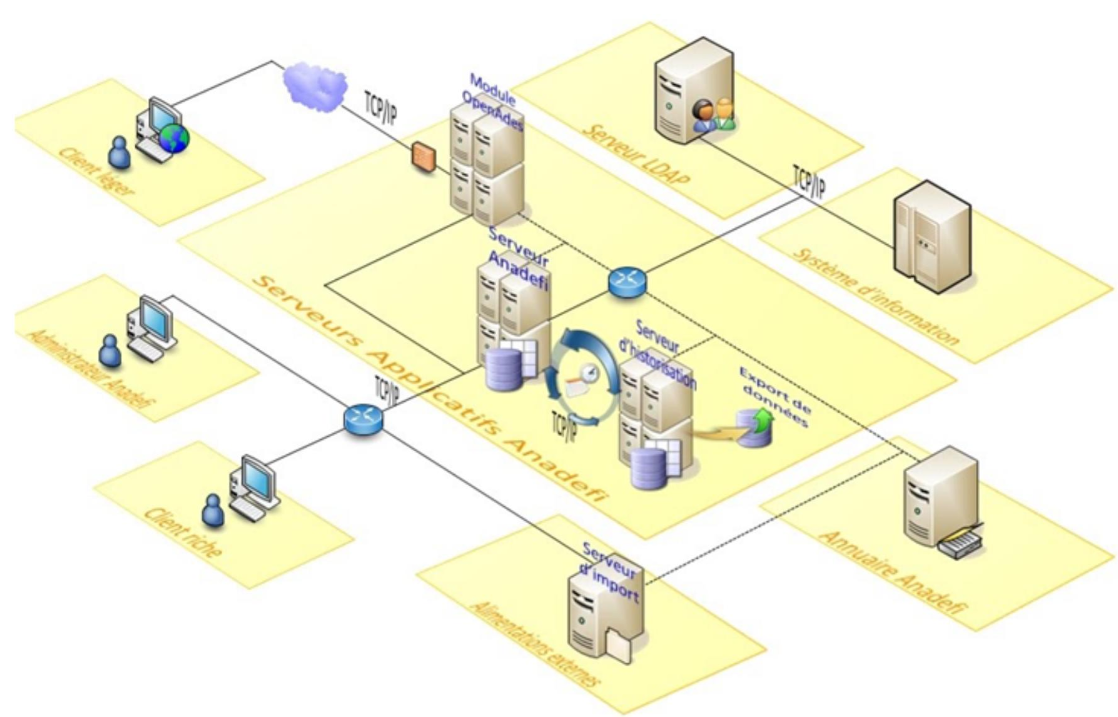
\includegraphics[scale=0.6]{resources/architecture.png}
\caption{Architecture Anadefi}
\label{ArchiAnadefi}
\end{figure}

\subsection{Gestionnaire d'instance}

Le gestionnaire d'instance est un outil qui va nous permettre d'avoir plusieurs instances du progiciel Anadefi avec chacun son propre serveur Ades, producteur et archivage.\\

L'avantage c'est qu'on peut avoir le paramétrage de chaque client et de switcher facilement d'une instance à une autre en un rien de temps.\\

Concrètement, tous les clients Anadefi n'ont pas les mêmes critères d'évaluations et de scoring en terme d'analyse financière et d'évaluation du risque. Pour pouvoir les administrer il aurait donc fallu installer le paramétrage d'un client d'abord, paramétrer, une fois terminé, désinstaller puis recommencer pour faire la même chose pour le deuxième, troisième client etc, on s'y perd très rapidement. C'est donc la raison pour laquelle on utilise le gestionnaire d'instance car il va nous permettre d'avoir plusieurs instances pour les différents clients Anadefi.

\subsection{Les outils Anadefi}

Il y a plus d'une vingtaine d'outils qui permettent de paramétrer le progiciel Anadefi.
Chaque serveur a ses propres outils pour paramétrer et configurer ces derniers.\\

Pour créer ou modifier un paramétrage on passe par un outil qui sert à administrer la base de données Anadefi qui est "Admin2000.exe". Il est destiné à un administrateur fonctionnel en charge de renseigner les nomenclatures des différentes listes déroulantes de l’application cliente, le paramétrage des grilles d'analyse, des grilles de saisie, les documents de sortie EDW\footnote{c'est un document similaire à Word}, les systèmes de cotations et de scoring.\\

Une fois que le paramétrage est crée ou modifié, on lance un autre outil "packager.exe" qui va créer un fichier avec l'extension .ppa qui contiendra toutes les nomenclatures, grilles d'analyse, de saisie, EDW etc, qu'on a paramétré au préalable sur admin2000.exe.\\

Pour que ce paramétrage soit effectif, on va utiliser un autre outil appelé "deployer.exe" qui va appliquer ce .ppa à l'instance correspondante, toutes les configurations faites par l'administrateur fonctionnel.\\

Une fois le paramétrage déployé, on va utiliser un dernier outil qui va mettre en production ce paramétrage, c'est l'outil "devprod.exe". Une fois utilisé, le paramétrage fait par l'administrateur est en place.\\

Il y a encore plusieurs outils qui permettent de paramétrer ou d'administrer le progiciel Anadefi.



\section{Missions et Objectif}

\subsection{Missions}
Durant mes deux mois de stage, j'avais comme mission principale de paramétrer le progiciel Anadefi et cela, pour les quatre projets sur lesquels j'ai pu travailler.\\

J'avais donc plusieurs tâches à accomplir pour mener ma mission à bien comme participer tout ou partie à la rédaction de spécifications fonctionnelles, participer aux ateliers fonctionnels (audio ou sur site), rédiger les comptes rendus, participer à la conception et à la création de scripts "métier" et effectuer les tests de toutes les modifications apportées ou encore tester les scripts.
Toutes ces tâches sont des étapes des projets sur lesquels j'ai travaillé et je vous détaillerai chaque étape avec précision ultérieurement dans ce rapport.\\


\subsection{Objectif}
L'objectif était de répondre au mieux aux besoins des clients, que cela soit d'ajouter un nouveau paramétrage, en modifier un existant ou encore apporter une correction sur un des paramétrages déjà en place. L'export de données client, entre aussi dans le cadre de ma mission en tant que consultant fonctionnel.\\




\section{Environnement de travail}


\subsection{Présentation de l'équipe}

Le pôle service Anadefi est composé de :
\begin{itemize}
\item Alexandre LIGER : Responsable Pôle Service Anadefi
\item Irenee MANGENOT : Consultant / Chef de projet
\item Simon LABATUT : Presales Manager
\item Haseeb CHAUDHRY : Stagiaire consultant fonctionnel\\
\end{itemize}

Irenee MANGENOT est située à Montpellier dans les locaux de Sopra Banking Software (ex O.R System) tandis que Alexandre Liger et Simon LABATUT font régulièrement du télétravail mais se sont rendu très disponible pour me rejoindre sur Paris (La défense ou Kléber) au moins deux fois par semaine.
Me concernant, j'étais dans les locaux de La Défense (tour Manhattan) ou dans les locaux de Kléber en fonction de la venue d'Alexandre LIGER et/ou de Simon LABATUT.\\

Durant ce stage, j'ai donc travaillé la majeure partie de mon temps en autonomie et à distance bien que, je pouvais contacter mon tuteur ou l'un des responsable projets à tout moment quelle que soit ma demande.

\subsection{Méthodes de travail}

La méthodologie de travail utilisée est le cycle en V. La première étape de cette méthode permet de détailler le service jusqu'au début de sa réalisation. Il comprend donc les étapes suivantes: L'expression des besoins du client, l'analyse, écriture des spécifications générales et fonctionnelles. Une fois la réalisation du service achevé, on effectue une série de tests: test fonctionnel, d'intégration et enfin de validation qui va déterminer si le service répond au besoin exprimé par le client. Après cela, nous procédons à la livraison de la recette.\\

Sur tous les projets j'ai donc utilisé cette méthodologie et réalisé ou pris part a certaines de ces étapes.\\

Pour mon travail, un suivi quotidien était organisé sous forme de réunion via Skype/Teams avec mon tuteur. Je parlais de mon avancement effectué la veille, de mes éventuelles difficultés rencontrées. Je lui montrais mon travail et ce que j'allais faire durant la journée.\\

Certains aspects de la méthode agile ont pu être appliqués après ma demande auprès de mon tuteur comme le sprint planning meeting, le daily stand-up et la revue de sprint bien que la notion de sprint soit absente.

Malgré que je sois seul, il y avait toujours quelqu'un de disponible pour répondre à mes questions et valider le paramétrage ou l'écriture des spécifications.\\

Lorsqu'un paramétrage était terminé, j'envoyais le nouveau fichier de paramétrage à mon tuteur ou au responsable du projet en question pour qu'ils puissent à leur tour vérifier et le tester puis l'envoyer au client.\\
\section{Déroulement du stage}
\subsection{Formation}

Les deux premières semaines de mon stage étaient dédiées à ma formation au progiciel Anadefi. Durant la première semaine, mon tuteur m'a présenté à son équipe, il m'a également présenté les locaux, comment est-ce qu'ils travaillaient tous ensemble et la présentation du progiciel entre autres.\\

La deuxième semaine, ma formation a eu lieu à Montpellier. J'ai tout d'abord installé un système de base de données (SQLServer) qui contenait toutes les données de leurs clients Anadefi. Par la suite, j'ai installé le progiciel et on m'a expliqué son mode de fonctionnement. La formation était très théorique car la pratique allait venir directement en travaillant sur les projets.

\subsection{Apprentissage par la pratique}

Dans mon cas, la meilleure façon d'apprendre était par la pratique car on applique directement les tâches, les concepts qui ont été expliquées juste avant. Et puis c'est aussi un très bon moyen d'apprendre quand les tâches sont plus ou moins répétitives comme cela a été le cas pour deux des quatre projets sur lesquels j'ai travaillé. Et puis pour être complètement formé au progiciel Anadefi il faut en moyenne trois mois, qui correspond quasiment à la durée de mon stage donc cette méthode était bien la meilleure solution.

\subsection{Planification} 

Avant même mon arrivée, mon tuteur avait déjà prévu les projets sur lesquels j'allais travailler, en fonction de la difficulté, du fait que je ne sois pas issu du monde de la finance, de mes points forts qui sont la programmation dont faire des scripts, que je puisse aussi travailler en autonomie et de la durée en jour pour que je puisse voir plusieurs aspects du rôle de fonctionnel.


\section{Les projets}

J'ai donc, comme expliqué précédemment, travaillé sur quatre projets au moment de l'écriture de ce rapport.
Le premier est la SIB\footnote{Société Ivoirienne de Banque}, Palatine, Banque Dupuy de Parseval et ABE\footnote{Agricultural Bank of Egypt}.

\subsection{SIB}

La Société Ivoirienne de Banque est une des filiales de groupe bancaire marocain Attijariwafa Bank. C'est l'une des banques les plus importantes en côte d'ivoire.\\

La mission était d'ajouter une nouvelle note système qui permettrait d'évaluer le risque crédit sous forme de notation en se basant sur une note système existante et en rajoutant un questionnaire.\\

Il fallait donc dans un premier temps créer un EDW. Un EDW est un document de type Word propre à Anadefi qui permet de relier les réponses des utilisateurs à la grille de notation correspondante.

\begin{figure}[h]
\centering
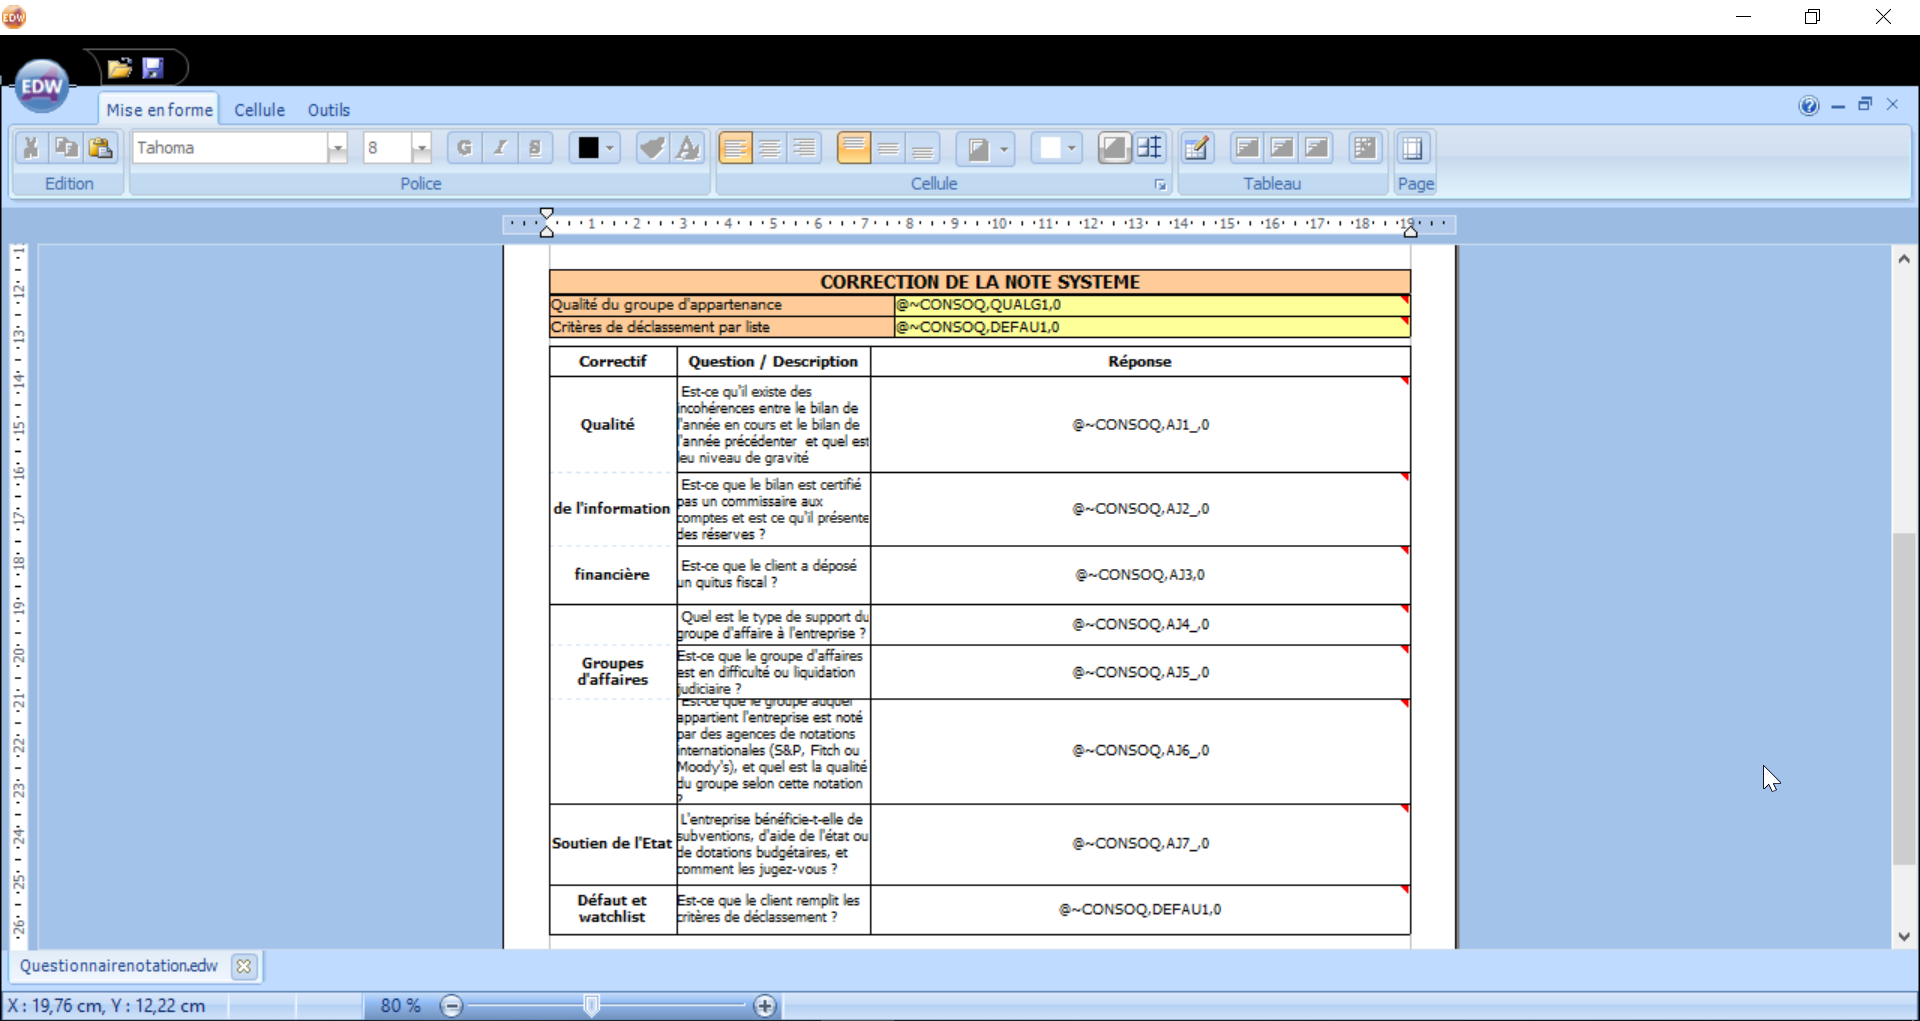
\includegraphics[scale=0.5]{resources/edw.png}
\caption{EDW questionnaire}
\label{edwSIB}
\end{figure}

Les réponses aux questions seront donc reprises grâce aux codes que vous pouvez voir dans la colonne "Réponse" et c'est dans l'outil Admin2000.exe qu'on va les traiter.\\

Dans l'outil Admin2000.exe on sélectionne la grille de cotation en question. Pour relier les questions et réponses aux EDW on utilise le code de la grille puis le code de la cellule.
Chaque réponse à une valeur différente, cette valeur a été exprimée par le client dans le cahier des charges. Pour attribuer la valeur à la réponse sélectionnée il faut faire des fonctions booléennes comme dans l'exemple suivant : 


\begin{figure}[ht]
\centering
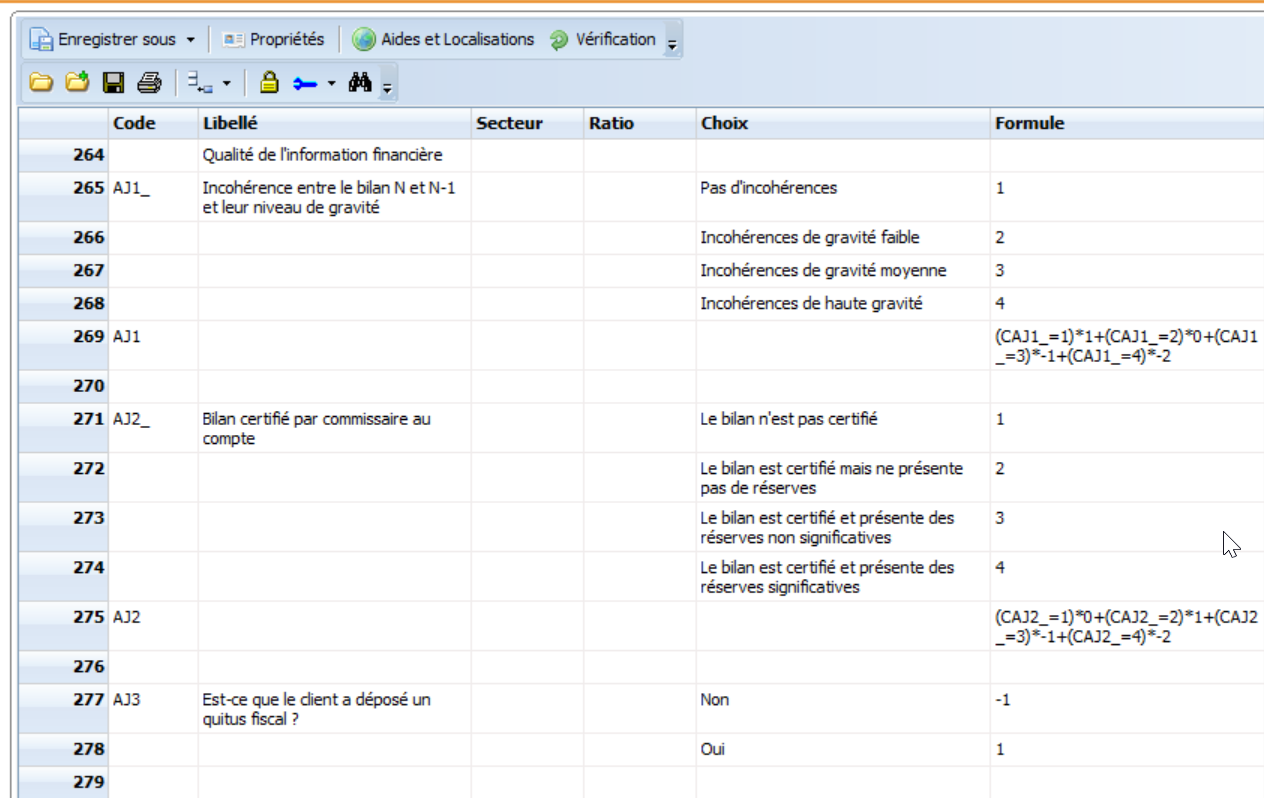
\includegraphics[scale=0.5]{resources/fctBoolAdmin.png}
\caption{Fonction booléen}
\label{fctBool}
\end{figure}


On trouve donc les réponses à une question posée. Chaque question est dans un ordre précis accompagnée d'un numéro. Le numéro de question est multiplié par la valeur de la question (qui nous a été donnée par le client) si et seulement si elle est cochée dont l'intérêt d'utiliser les fonctions booléens.\\

Une fois que toutes les questions sont reliées, on va additionner le tout pour obtenir un résultat numérique et c'est ce résultat qui va constituer une partie de la note. Cela se fera dans la grille de notation.

\begin{figure}[ht]
\centering
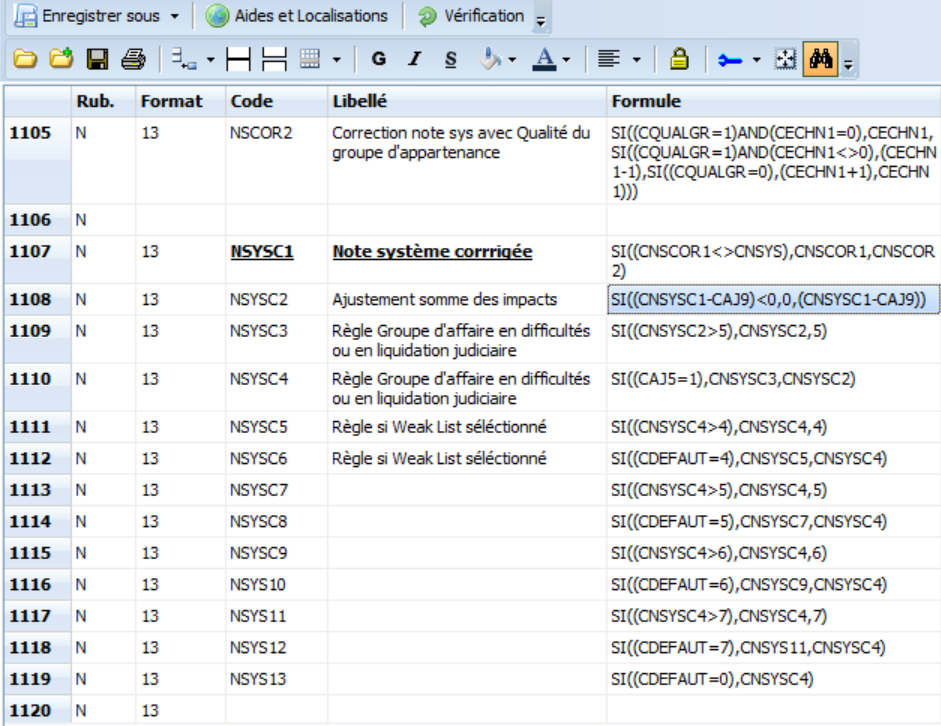
\includegraphics[scale=0.6]{resources/grille_notation.png}
\caption{Grille de notation}
\label{grCot}
\end{figure}

Dans cette grille, nous allons mettre en place toutes les conditions exprimées par le client qui feront qu'en fonction de la réponse de chaque question on obtienne une note. Par exemple si la note obtenue en remplissant le questionnaire vaut 3 mais qu'on a répondu "non" à la question 4 alors on prendra la pire note entre la note système actuelle et la note F\footnote{Une notation exprimée par le client}. Il y a pleins d'autres conditions de la sorte mais je ne vais pas détailler d'avantages, si besoin, se référer à l'annexe 1.\\

Une fois terminée, il a fallu tester une vingtaine de cas et en cas d'anomalie il fallait naturellement corriger puis retester. Une étape assez longue et difficile car c'est un travail qui demande beaucoup de rigueur et de patiente.\\

Après avoir testé, grâce à l'outil packager.exe je récupère le nouveau paramétrage l'envoi au responsable projet qui va valider et livrer la recette.\\

Sur ce projet, il n'y avait pas de problème en particulier, mais le temps de comprendre à quoi correspond chaque interface, comment écrire le plus clairement et le plus proprement possible les règles de gestion, ce n'était pas si simple surtout quand c'est la première fois qu'on fait ce genre d'exercice.


\subsection{Palatine}

Palatine est l'une des plus anciennes banques françaises encore en activité. Elle est de taille intermédiaire et elle est au service des entreprises de taille intermédiaires et de la gestion de patrimoine. Elle fait partie du groupe BPCE.\\

La banque de Palatine a contacté Sopra Banking Software pour une prestation d'extraction de données depuis leur base de données Anadefi car ils souhaitaient migrer leurs données vers un nouvel outil qui a été développé en interne par le groupe.\\

Ce qui était prévu initialement, c'était de créer trois fichiers en .ini à partir de l'outil "DefExport.exe", qui allaient ensuite être insérés dans l'outil "MoteurDexport.exe". Cet outil va par la suite, générer les trois fichiers en .csv contenant toutes les données financières demandées par Palatine.\\

La première étape est donc de monter un environnement Anadefi similaire à celui de Palatine, ce qui comprend la même version du logiciel, la même base de données, avec le même paramétrage entre autre.\\

La deuxième étape était de créer les fichiers .ini à l'aide de l'outil "DefExport.exe" dans lesquels on va indiquer les grilles financières que l'on souhaite extraire, la date des exercices, les données financières à partir des codes fournis et toute autre condition.\\

La troisième étape était donc de tester si les fichiers en .ini crées sont correctes et s'ils exportent bien les données demandées. C'est donc à ce moment que nous nous sommes aperçu qu'il y avait un gros soucis de volumétrie et que trois fichiers en .ini ne suffisaient pas pour exporter la totalité des données demandées.\\

Nous avons donc décidé d'appliquer plusieurs filtres qui permettaient de repartir les données sur plusieurs fichiers. Le premier filtre était le découpage par grilles, il y avait cinq grilles différentes. Par la suite nous avons appliqué le découpage par bureau en fonction du nombre de dossiers. Certains bureaux étaient composés d'environ 2000 dossiers et d'autres à peine une centaine, il a donc fallu donc essayer de repartir au mieux les bureaux sur les fichiers pour trouver un bon équilibre, sans qu'un fichier soit beaucoup trop volumineux par rapport à un autre. Prendre uniquement les cinq derniers exercices et prendre uniquement les exercices dont le numPartenaire\footnote{un numéro d'identifiant unique} est renseigné. En découpant par tous ces filtres nous sommes passés de trois à vingt.\\

Comme mentionné plus haut, c'est avec l'outil "DefExport.exe" qui permet de créer les fichiers d'extraction en .ini.
Dans cet outil on va définir le nom du fichier, le séparateur qui sera utilisé dans le .csv, la sélection d'une ou plusieurs grilles, la date d'échéance des exercices, le nom du fichier .csv généré et son contenu, les différents filtres qui sont demandés par le client et toute information qui serait dans le fichier .ini et dans le .csv. Au moment de la sélection des codes, il faut créer un champs dans lequel on va indiquer le nom du champs, le type de la donnée et la valeur de la donnée.

\begin{figure}[ht]
\centering
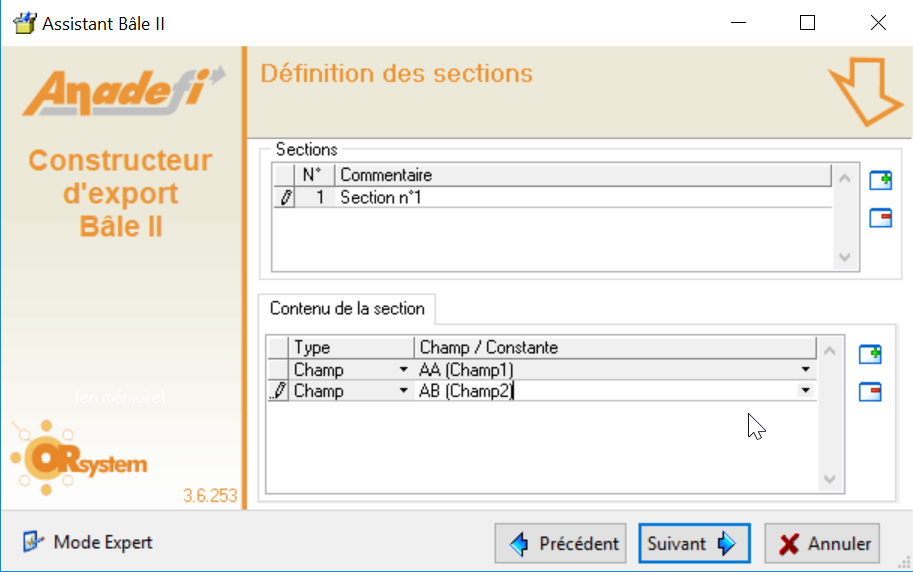
\includegraphics[scale=0.6]{resources/champ1.png}
\caption{Création des champs}
\label{champ1}
\end{figure}

\begin{figure}[ht]
\centering
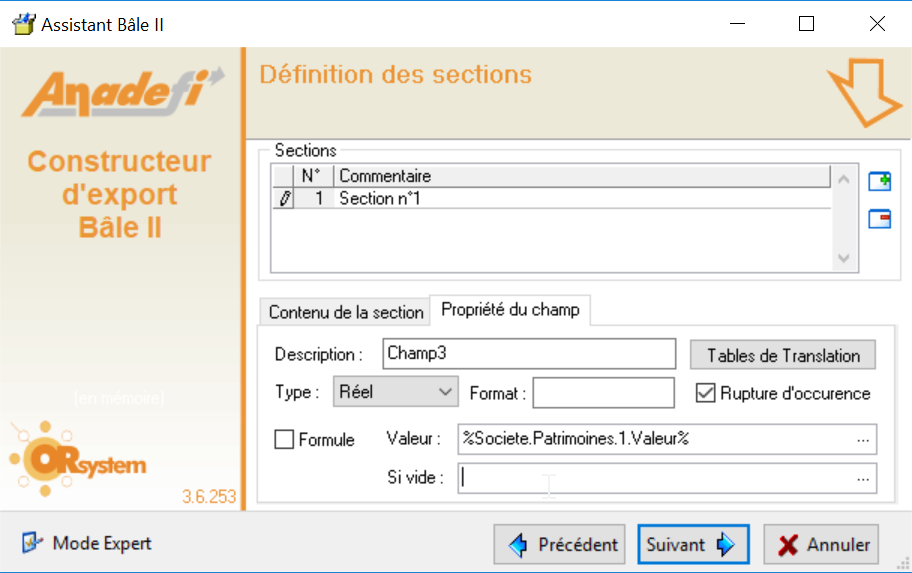
\includegraphics[scale=0.6]{resources/champ2.png}
\caption{Renseignements des champs}
\label{champ2}
\end{figure}

Le problème était qu'il fallait répéter cette action pour chaque champ c'est-à-dire 321 multipliées par 20 ce qui est très très long et le risque d'erreur est très élevé.\\

J'ai donc décidé de faire un script en Python. Pour créer un fichier j'aurai pu prendre n'importe quel autre langage mais j'ai choisis le Python pour sa simplicité syntaxiquement parlant mais aussi, le fait que je n'ai pas pratiquer du Python durant cette année contrairement au langage Java.\\

J'ai tout d'abord fait une requête SQL pour pouvoir afficher, copier et coller tous les codes qui allaient être utilisés. Par la suite, j'ai utilisé une expression régulière pour que les codes puissent être entre guillemet comme dans la figure suivante :


\begin{figure}[ht]
\centering
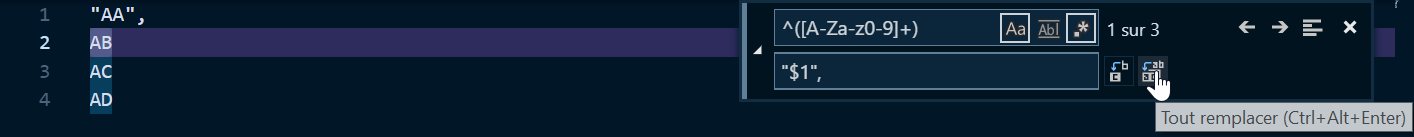
\includegraphics[scale=0.6]{resources/regex.png}
\caption{Expression régulière}
\label{regex}
\end{figure}

J'ai donc créé une liste contenant les codes en rajoutant des crochets. J'ai ensuite effectué le même procédé avec les différents bureaux. Arrivé à ce moment, j'avais tous les éléments pour faire mon script. J'ai donc eu à faire deux boucles imbriquées, une condition et une fonction qui me permet de créer des fichiers pour faire mon script. Pour tester les fichiers .ini créent à partir de mon script, j'ai dû les tester directement dans l'outil qui permet de faire l'extraction "Moteurexport.exe" si le fichier .ini ne généré pas d'erreur ni d'avertissement et qui me donnait en sortie mon fichier .csv avec des données alors le script était bon. Pour tester, je n’avais plus vingt fichiers .ini mais seulement quelques lignes de codes que j'ajustais au fur et mesure des erreurs trouvées dans les fichiers générés. Au final j'ai gagné beaucoup de temps et puis même à l'avenir pour un autre projet d'extraction mes scripts sont réutilisables et facilement ajustable.

Une fois terminée, j'ai écrit une documentation indiquant les noms des fichiers .csv qui seront générés, en fonction de leur contenance : les grilles, bureaux, le type de bilan, le nombre de dossiers à extraire pour chaque fiche et pour finir l'intitulé des codes pour qu'ils puissent savoir à quoi correspond une valeur présente dans le .csv.

\subsection{ABE}

Agricultural Bank of Egypt est une banque de la filiale National Bank of Egypt qui a été fondé en 1902.
Elle est spécialisée pour les particuliers initialement issus de l'agriculture mais s'est diversifié au fur et mesure des années.\\

Nous avions reçu une offre commerciale pour une modification et correction d'un paramétrage existant.
Le responsable de projet a rédigé la proposition commerciale. J'avais pour mission d'écrire les spécifications à partir du cahier des charges.\\

Ce cahier des charges était entièrement en anglais, il n'y a aucun interlocuteur qui parle français chez ABE. Cela n'a pas été un problème car j'ai une certaine aisance en anglais. À l'aide de mon responsable j'ai donc écrit en français chaque besoin exprimé par le client. Je l'ai rédigé en français car c'est un document qui restera en interne au sein du Pôle Service d'Anadefi. Vous trouverez en annexe une partie de la spécification. À ce jour, on attend que l'ABE signe la proposition commerciale pour pouvoir démarrer les travaux.



\subsection{Banque Dupuy de Parseval}

Banque Dupuy de Parseval est une banque, tout comme Palatine du groupe BPCE. Elle est présente dans la région du Languedoc - Roussillon et est au service principalement des entreprises de la région.\\

Pour les mêmes raisons que la banque de Palatine, elle souhaite extraire tous ces données de la base Anadefi pour les importer dans l'outil développé par le groupe BPCE.\\

Pour ce projet, j'ai écrit une grosse partie de la proposition commerciale car ayant travaillé sur Palatine juste avant, je connaissais les différentes étapes, prérequis, la prestation en elle même et les éléments à livrer. Dans cette proposition, j'ai écrit les différentes étapes de la prestation demandée.
La première était de définir l'objectif de la prestation. Ensuite définir les modalités qui doivent être réalisées et celle qui ne le seront pas. Les prérequis de cette extraction, dans ce cas étaient que BDP fasse une sauvegarde et un recalcule de leur base de données Anadefi. Un résumé des différentes tâches sous formes de tableau indiquant qu'est ce que le client doit fournir ou être livré et ce qu'Anadefi doit fournir ou être livré. Concernant la partie estimation du délai de la prestation, les coûts, les clauses et tout ce qui est d'ordre de l'administratif ont donc été écrites par le responsable de projet. \\

Contrairement à Palatine nous n'avons pas eu de problème de volumétrie par conséquent, on n'a pas appliqué de filtre car on ne découpait pas les données.\\

Concernant l'écriture des fichiers .ini, j'ai donc récupéré le script que j'avais fait pour la banque de Palatine, j'ai fait quelques ajustements pour que le script génère les bons fichiers .ini et donc les bonnes données dans le .csv. La phase de test a été beaucoup plus longue à cause du temps d'extraction car contrairement à Palatine, j'avais toute la base de données sur ma machine.\\

Une fois les tests effectués j'ai envoyé les fichiers .ini au responsable de projet qui par la suite, a vérifié et testé de son côté. J'ai donc entre temps écrit une documentation indiquant le contenu des fichiers.




\section{Conclusion}

Après avoir effectué plus de la moitié de mon stage, j'en suis déjà très satisfait. De part l'accueil que j'ai reçu, la patiente qu'ont eu mes collègues lors de mes différentes formations, de m'offrir la possibilité de pouvoir prendre des initiatives, de l'attribution des projets qui correspondent plus à mon profil et de leur confiance.\\

J'ai accepté une mission qui me donnait la possibilité de découvrir autre chose que la programmation, c'est le fonctionnel. Faire partie de l'équipe fonctionnelle me permet de voir comment est ce qu'ils interagissent avec les différents services de l'entreprise dont les développeurs et même le contact client. Au-delà des compétences techniques que j'ai acquises sur le progiciel Anadefi, j'ai appris une chose essentielle, c'est que la communication est un facteur déterminant pour mener un projet à bien. En tant que futur développeur c'est une compétence essentielle surtout dans un cadre agile.\\

Par ailleurs j'ai pu appliquer certains concepts de la méthodologie agile comme les daily stand up et les test d'acceptance cependant le cycle en V correspond mieux au bon fonctionnement de l'équipe fonctionnelle.


\section*{Liste des annexes}
\begin{enumerate}
  \item \Large{Spécification de la SIB}
  \item \Large{Spécification pour l'ABE}
  \item \Large{Tableau des tâches BDP}
  \item \Large{Listes des outils Anadefi}
\end{enumerate}
\section*{1. Spécification de la SIB}


\paragraph{I)	Groupe d’affaire en difficultés ou en liquidation judiciaire\\ }
Si la réponse de la question Q5/ dans le questionnaire est "oui" alors prendre la pire note entre La note système ajusté intermédiaire et la note "F".
Sinon alors prendre La note système ajusté intermédiaire.\\


\paragraph{II)		Défaut\\}

\begin{itemize}
    \item Si le client remplit les critères de déclassement en Weak List alors prendre la pire note entre La note système ajusté intermédiaire et la note " E ".
    \item Si le client remplit les critères de déclassement en Watch List 2 alors prendre la pire note entre La note système ajusté intermédiaire et la note " F ".
    \item Si le client remplit les critères de déclassement en Watch List 1 alors prendre la pire note entre La note système ajusté intermédiaire et la note " G ".
    \item Si le client remplit les critères de déclassement en CDL alors prendre la pire note entre La note système ajusté intermédiaire et la note " H ".
    \item Sinon alors prendre La note système ajusté intermédiaire.
\end{itemize}


\section*{2. Spécification de l'ABE}


Ajout de données dans le IDC module : Main data et Grading Data. Nouveau champs "External Auditor Name" et l'exporter dans IDC\\

Nouvel onglet dans 'Analysis - Rating' nommé "Grading Approuved 'Yes/No'. Cet onglet doit afficher 'YES' une fois que la notation est validée. Si il y a un changement dans le questionnaire qualitatif ou quantitatif, il doit afficher 'NO'.\\

\begin{itemize}
\item Mettre à jour la liste des valeurs de "override reason" ajouter/supprimer les valeurs.
\item Évaluer l'impact des données manquante après la migration en ajoutant un historique dans Anadefi.
\item j'ai pas compris.
\item Ajouter un contrôle quand le user choisi "override reason" pour que le champs ne soit pas vide.
\item (Changer)? l'affichage de la zone de notation du système.
\item Mettre à jour/changer la liste déroulante des status des clients.
\end{itemize}

\section*{3. Tableau des tâches BDP}

\Large{À chaque tâche correspond une lettre :\\ }

\begin{itemize}
\item "\textcolor{red}{R}" : la Partie à qui est affectée la réalisation de la tâche.
\item "\textcolor{red}{P}" : la Partie qui doit assister l’autre Partie dans la réalisation de sa tâche. Lorsque cette tâche est attribuée au Client, il appartient au Client de transmettre au Prestataire les éléments nécessaires à la réalisation de la tâche considérée. Lorsque cette tâche est attribuée au Prestataire, il appartient au Prestataire de réaliser un transfert de compétence au bénéfice du Client.
\item "\textcolor{red}{V}" : la Partie qui doit procéder au contrôle des résultats des tâches.\\
\end{itemize}

\begin{figure}[h]
\centering
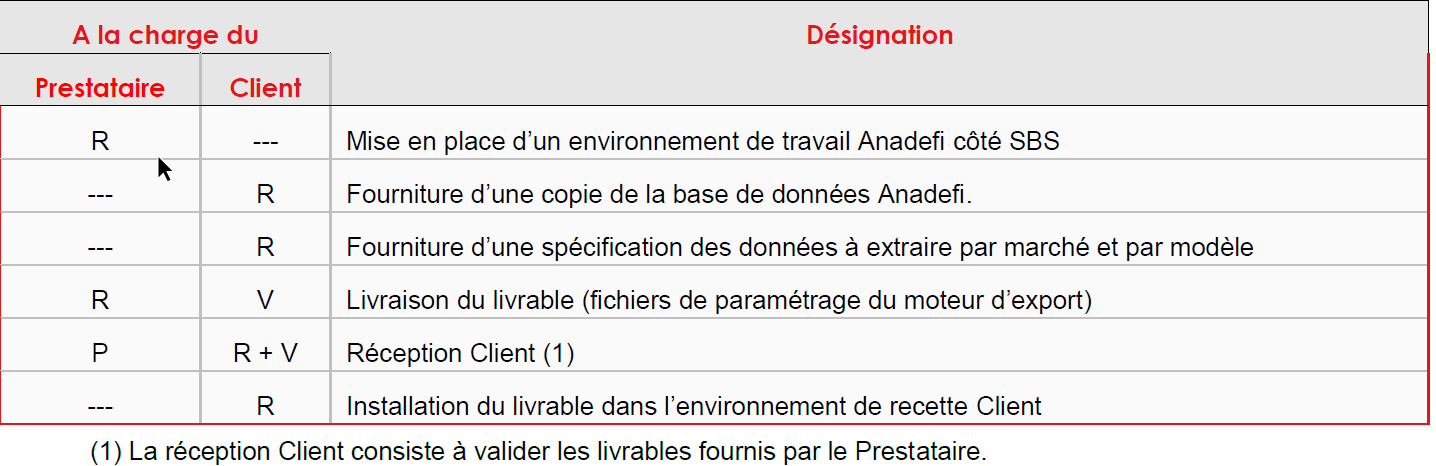
\includegraphics[scale=0.6]{resources/tachesBDP.png}
\caption{Tableau des tâches}
\label{tbl BDP}
\end{figure}
\section*{4. Les outils d'Anadefi}

\begin{description}
    \item[Gestionnaire d'instance :] Permet d'avoir plusieurs instances clients sur une même machine. 
    \item[Packager :] Permet d'exporter toute la configuration d'une instance en un fichier avec l'extension .ppa.
    \item[Deployer :] Permet d'appliquer un nouveau paramétrage à partir d'un fichier .ppa.
    \item[Devprod :] Permet de mettre en production le paramétrage appliquer au préalable avec l'outil Deployer.
    \item [Admin2000 :] Permet de configurer la base de données et de créer, modifier ou encore corriger un paramétrage. 
    \item[DefExport :] Permet de créer les fichiers avec l'extension en .ini qui serviront à l'extraction pour l'outil MoteurExport.
    \item[MoteurExport :] Génére le fichier en .csv(ou autre extension) à partir des fichiers .ini créer avec l'outil DefExport.
\end{description}
\section*{Webographie}


https://www.soprabanking.com\\
http://www.orsystem.com\\
https://www.soprasteria.com/fr/investisseurs/a-item\\
https://www.python.org/\\
https://code.visualstudio.com/\\
Documentation interne d'Anadefi\\
Capture d'écran réalisé par moi même\\






\end{document}